%!TEX root = ../dissertation.tex

\chapter{Introduction}
\label{chapter:introduction}

\section{From Paper to Bits}
Through the years, computers have been taking more ground in the field of architecture.
It began with the appearance of Sketchpad\cite{Sutherland:1964:SPM:800265.810742} in the 60s that showed that computers could be used to create drawings interactively.
After the appearance of desktop computers, drafting software like AutoCAD popularized \gls{cad} in architecture.
As opposed to drawing by hand, using computers to create these drawings allowed architects to make changes without having to redraw their drawings, therefore saving them much time.

As computers became powerful enough to display 3D graphics and 3D modeling started to appear, it became possible to model buildings in the computer and preview them using interactive 3D views.
This has allowed \gls{cad} applications to be used to create visualizations and documentation for architectural projects.
However, modeling a building still requires repetitive and time-consuming tasks that are not trivial to accomplish using the functionalities provided by a 3D modeling software.


\section{Scripting}
The recognition of this problem has led to the emergence of programming for \gls{cad} applications.
By programming, the architect is able to describe what he wants to model in a program and let the computer create it for him.
On top of that, after writing the program, the process of creating the model and applying changes when needed is much faster than the manual equivalent.
As a result, the architect gets to do more in less time.

Some examples of programming languages being used in \gls{cad} applications include AutoLisp and Visual Basic for AutoCAD, GDL\cite{watson2009gdl} in ArchiCAD, Python and Grasshopper in Rhinoceros 3D, and Dynamo in Revit.


\section{Generative Design}
Having a faster and more flexible process for building 3D models allows the architect to explore more variations of a design, i.e., to explore a broader design space, since modeling is no longer too expensive and time consuming to do.
Designing by using programming to generate parts of the design is what is called \gls{gd}.
\gls{gd} allows computers to be used as a new medium for artistic expression\cite{Maeda:2001:DN:559503} that can be used by architects, as shown in \cite{terzidis2003expressive}.

Furthermore, as stated in \cite{leitao2014pushing}, using \gls{gd} as a new stage of the design process promotes a simpler handling of changes coming from uncertain design intents and emergent requirements which evolve as the understanding of the problem improves or as the project's needs change.
Programs are unambiguous parameterized representations of designs, which only need small changes to parameters or functions to express changes in designs.
In contrast, if 3D models are used, expressing changes in designs requires changing many more parts of those 3D models.
However, in order to create the programs that generate the architect's designs, the architect needs to have a programming environment, or \gls{ide}, that lets him write them and see their results.


\section{IDEs for Generative Design}
An \gls{ide} provides tools -- editors, compilers, debuggers, among others -- that let the architect create programs.
In the case of \gls{gd} \glspl{ide}, there are specific requirements that need to be fulfilled to make them useful for exploration of \gls{gd}, since these \glspl{ide} have to support the architect while he creates programs and explores design possibilities.
First of all, they have to be able to display geometric results, otherwise, the architect will not be able to see what his programs generate.
Secondly, the architect needs to be able to see the effects from changes to parameters or to any part of the program.
This will require the environment to run programs fast, generate results, and display them to the architect, thus giving him immediate feedback.
Apart from this, the environment also needs to make it easy for the architect to build his program and correct the bugs that might appear.
It may do so by showing him the available functions or by highlighting results from a given part of a program.

Examples of \gls{gd} \glspl{ide} include Grasshopper 3D\footnote{\url{http://www.grasshopper3d.com/} (last accessed on 10/10/2016)} for Rhinoceros 3D\footnote{\url{https://www.rhino3d.com/} (last accessed on 10/10/2016)}, Dynamo\footnote{\url{http://dynamobim.com/} (last accessed on 10/10/2016)} for Revit\footnote{\url{http://www.autodesk.com/products/revit-family/overview} (last accessed on 10/10/2016)}, and Rosetta\cite{de2012modern}.
Up until now \gls{gd} \glspl{ide} have been desktop applications, which bring some disadvantages.


\section{Disadvantages of Current CAD Applications}
The first disadvantage of current \gls{cad} applications is that they need to be installed.
Like so, they are not readily available on every computer, which limits their potential for expressing ideas.

The web has seen a big increase in popularity which has become even stronger by the standardization of both new and existing web technologies such as HTML5\cite{hickson2011html5} and WebGL\cite{marrin2011webgl} that allow web applications, accessed using web browsers, to achieve user experiences on par with desktop applications.
This has led to the creation of many web application counterparts of common desktop applications.
For example, office productivity tools like Microsoft Word, Excel and PowerPoint have seen the appearance of their web application counterparts when Microsoft Office 365 appeared.
Furthermore, complete \gls{cad} web applications have also appeared.
One example is OnShape\footnote{\url{https://www.onshape.org} (last accessed on 10/10/2016)}, a \gls{cad} application for Product Design/Engineering completely accessible from the web browser.

The second disadvantage of current \gls{cad} applications is that their performance is not adequate for \gls{gd}.
In order to do \gls{gd}, architects need to have an interactive environment where they can get feedback from their programs as fast as possible.
If the \gls{cad} application takes too long to generate the results, then the \gls{gd} environment will not be able to give this feedback.
This problem often reveals itself when working with Rosetta, as shown in \cite{Leitao2014illustrated}.
For example, when working on a building design like the one shown in Figure~\ref{fig:carmo:render}, the times for generating the model get high when a \gls{cad} backend like AutoCAD is used, as seen in Figure~\ref{fig:carmo:times}.
By looking at the figure, we can see that running times for \gls{cad} backends (AutoCAD, Rhinoceros and SketchUp) span at least a few seconds.
According to \cite{Leitao2014illustrated}, this problem comes from both the complexity of the \gls{gd} program, which can make running times grow beyond the limit for immediate feedback, and from the way \gls{cad} applications are implemented, which were designed to handle human interaction and not the volume of operations generated by \gls{gd} programs.
Like so, architects will have to wait before they see the updated results of their programs, thus, the immediate feedback is lost and it becomes harder to understand what the program is doing and how it does it.

\begin{figure}
	\centering
	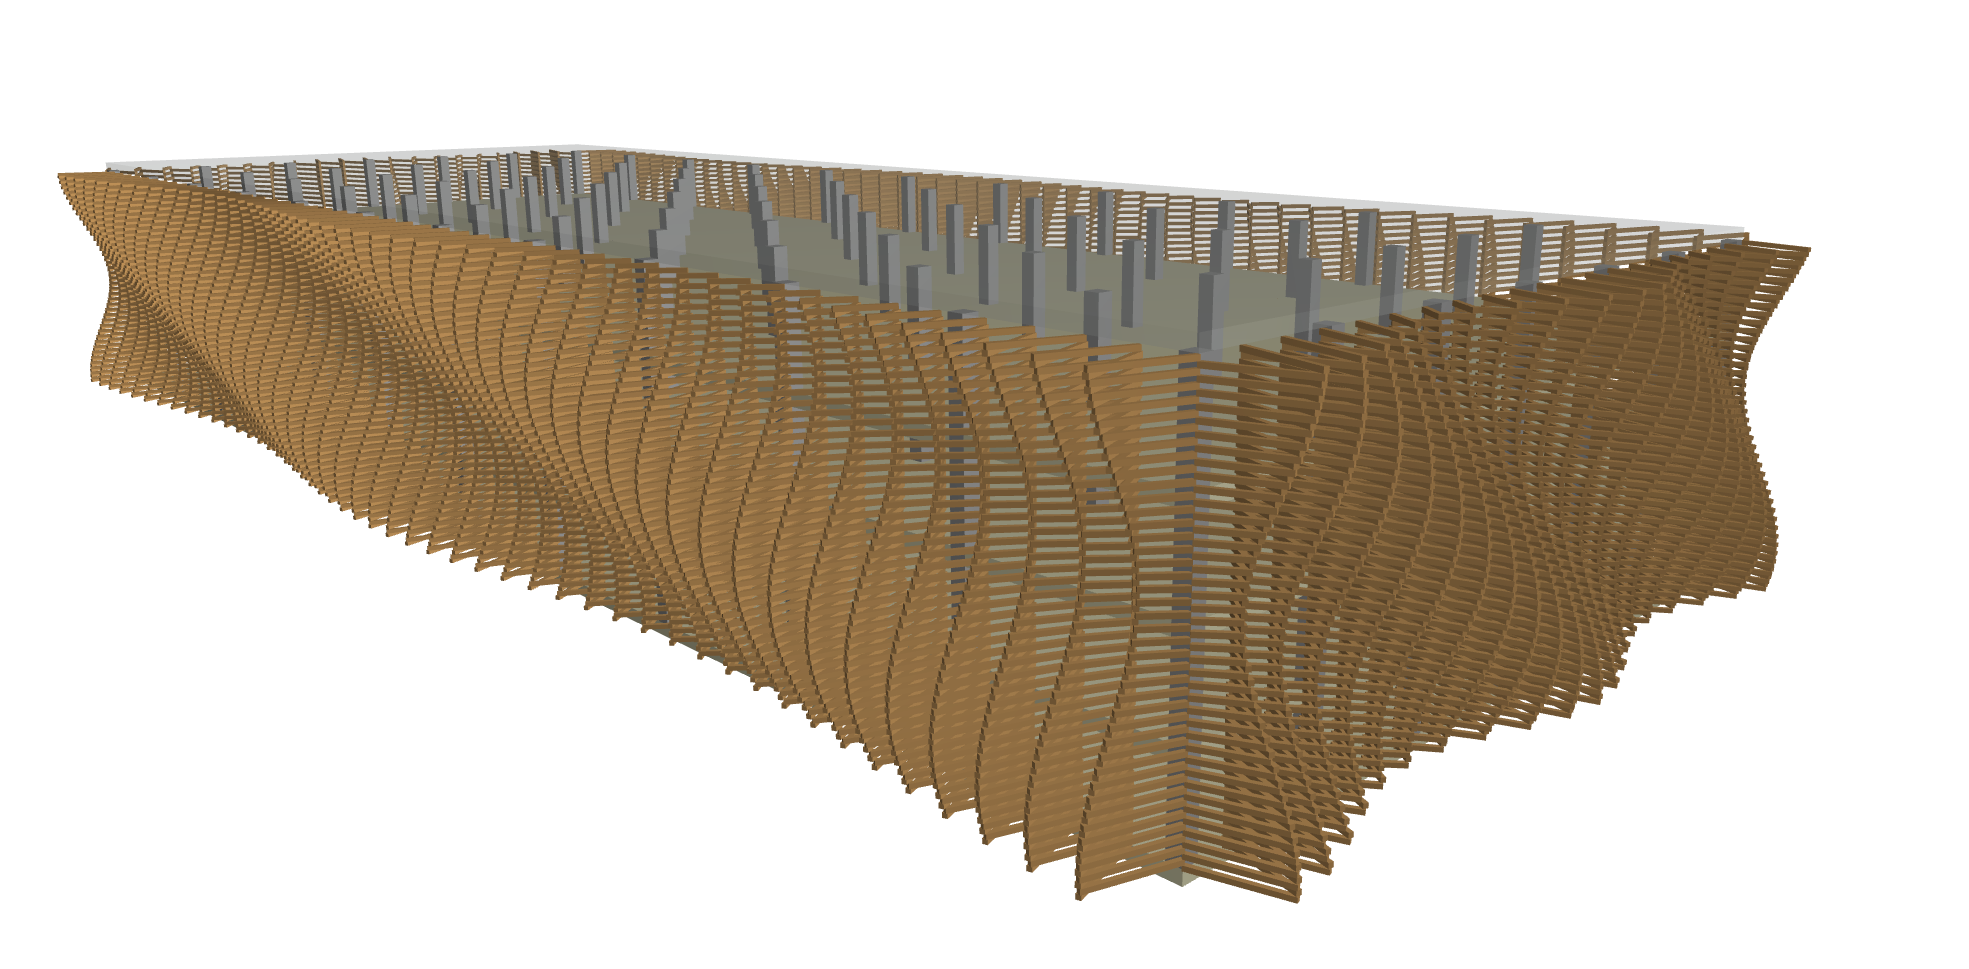
\includegraphics[width=0.8\textwidth]{images/carmo_render}
	\caption{Rendering of a building design made using \gls{gd}.}
	\label{fig:carmo:render}
\end{figure}

\begin{figure}
	\centering
	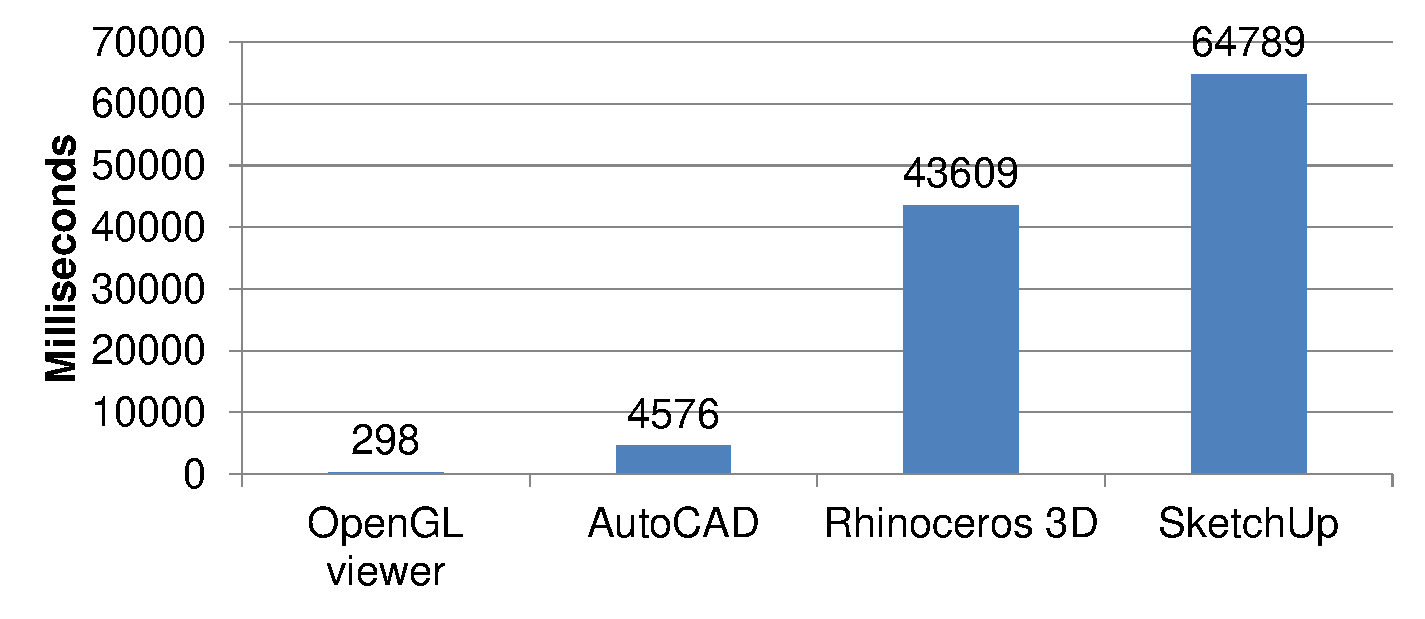
\includegraphics[width=0.8\textwidth]{images/carmo_rosetta_times}
	\caption{Generation times for different \gls{cad} applications using Rosetta.}
	\label{fig:carmo:times}
\end{figure}


\section{Goals}
A \gls{gd} \gls{ide} needs to have more \textbf{accessibility}, not requiring any installation and being available in any computer, and needs to be more \textbf{interactive}, letting architects explore \gls{gd} easily, giving them feedback and showing them the relationship between program and results.
Moreover, it needs to \textbf{integrate} easily with the \gls{cad} applications already used by architects, so they can still integrate their \gls{gd} experiments into their normal workflow.

This requires the implementation of a web page that harnesses the performance and graphical capabilities available in modern web browsers, and the implementation of a companion application for allowing models to be exported to traditional \gls{cad} applications.
In this way, architects can write their \gls{gd} programs and visualize the results without being chained to a particular computer, and can easily integrate results into their normal workflow by using the companion application.
We can summarize the contributions of this paper as follows:
- We describe a web page for creating \gls{gd} programs that makes use of immediate feedback and traceability mechanisms (Section A).
- We provide a way to integrate the web page \gls{ide} with other software tools used by architects (Section B).
- We show examples of use of the web page, namely, when creating programs and when exporting to desktop \glspl{cad} (Section C).
- We compare the web page with Rosetta and OpenJSCAD by measuring the times for running a program and displaying its results (Section D).
